The OutComponent component encapsulates an out-going command or an out-going report. This component enforces the generic behaviour that is common to all out-going commands and reports irrespective of their type and it provides access to their attributes.

The OutComponent component – like all other CORDET Framework components – is an extension of the Base Component of section \ref{sec:BaseCmp}. Behaviour which is specific to the OutComponent component is defined by the state machine shown in figure \ref{fig:OutComponent} (the \textit{OutComponent State Machine}). This state machine is embedded within the CONFIGURED state of the Base State Machine. 

\begin{figure}[h]
 \centering
 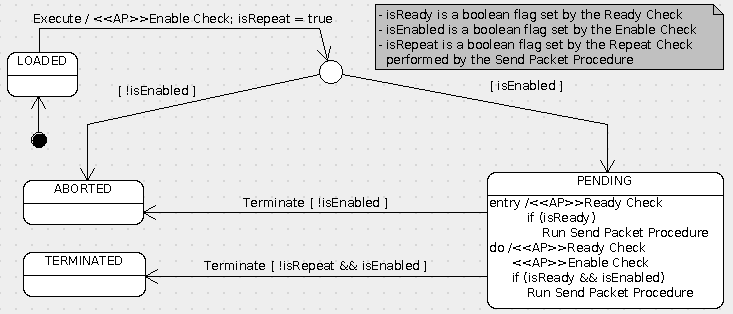
\includegraphics[scale=0.35,keepaspectratio=true]{OutComponent.png}
 \caption{The OutComponent State Machine}
 \label{fig:OutComponent}
\end{figure}

When the OutComponent is retrieved from its factory, it is initialized and reset (depending on the implementation, the \texttt{Reset} command may be issued either by the factory itself or by the user application). After the OutComponent has been successfully reset, the OutComponent State Machine is in state LOADED. The component then waits for the \texttt{Execute} and \texttt{Terminate} commands which are sent to it by its OutManager (see section \ref{sec:OutManager}). 

The OutComponent behaviour depends on the outcome of three checks. The \textit{Enable Check} verifies whether the command or report it encapsulates is enabled or not. If it is enabled, the check sets flag \texttt{isEnabled} to true; if it is disabled, it sets flag \texttt{isEnabled} to false. The \textit{Ready Check} verifies whether the command or report is ready to be sent to its destination. If it is ready to be sent, the check sets flag \texttt{isReady} to true; otherwise it sets the flag to false. The \textit{Repeat Check} verifies whether the command or report should remain pending after being sent to its destination. If the outcome of the Repeat Check is 'Repeat' (i.e. if the OutComponent should be sent to its destination again), flag \texttt{isRepeat} is set to true; if the outcome is 'No Repeat' (i.e. if the OutComponent should not bet sent again to its destination), flag \texttt{isRepeat} is set to false. The three check operations are adaptation points.

At each execution, the OutComponent performs the Enable Check and if this declares the OutComponent to be disabled, it makes a transition to state ABORTED. This marks the end of the OutComponent's lifecycle.

At each execution, the OutComponent has a chance to be sent to its destination. This is done when the OutComponent is declared to be both ready and enabled by its Ready Check and Enable Check. 

The sending operation is performed by the Send Packet Procedure of figure \ref{fig:SendPacket}. The Send Packet Procedure starts by performing the Update Action. Through this action, the OutComponent acquires the information it must transfer to its destination. By default, this action sets the time stamp attribute of the OutComponent. Applications may want to extend this action to load the values of the OutComponent parameters. For this reason, the Update Action is an adaptation point of the OutComponent.

The Send Packet Procedure then retrieves the destination of the OutComponent and then interrogates the OutStreamRegistry to obtain the corresponding OutStream (recall that, in an application, there is one instance of OutStream for each command or report destination). If an OutStream can be found (i.e. if the OutComponent's destination is valid), the procedure serializes the OutComponent to generate a packet which is then handed over to the OutStream. This ensures that the command or report will eventually be sent to its destination. The serialization process is an adaptation point. 

After serializing and handing over the OutComponent to its OutStream, the Send Packet Procedure performs the Repeat Check. This determines whether the OutComponent should be sent to its destination once more (the Repeat Check sets flag \texttt{isRepeat} to true) or whether its life is terminated (the Repeat Check sets flag \texttt{isRepeat} to true). In the latter case, the OutComponent will make a transition to TERMINATED.

If the OutStreamRegistry does not return any OutStream, then the procedure concludes that the OutComponent's destination is invalid and it reports the fact. In this case, the outcome of the Repeat Check is also forced to 'No Repeat' (i.e. flag \texttt{isRepeat} is set to false). 

\begin{figure}[h]
 \centering
 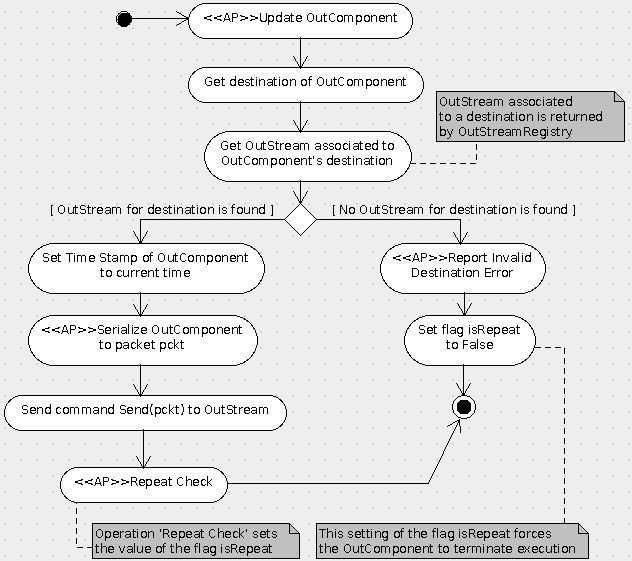
\includegraphics[scale=0.35,keepaspectratio=true]{SendPacket.png}
 \caption{The Send Packet Procedure}
 \label{fig:SendPacket}
\end{figure}

The OutComponent provides visibility over its internal state but it does not provide automatic notifications in case of changes in its internal state. The OutComponent provides access to the attributes of the command or report it encapsulates but it only predefines dummy values for them. The set and value of command or report attributes is therefore an adaptation point for the OutComponent. 

The default implementation of the Enable Check uses one of the services provided by the OutRegistry to determine the enable status of a command or report (see section \ref{sec:OutRegistry}).
